\chapter{\aicat\ Framework Design}
\label{design}

Framework design is a difficult task in general, because a
well-designed framework must allow for several kinds of
growth.\cite[p. 11]{fayad:99} The framework interface must be
usefully applied to several different use cases, including ones that
the framework designer may not be able to foresee.  The framework must
also be extensible by subclassing, and must therefore have enough
structure that the relationships among classes are well-defined, yet
flexible enough that the application developer can make appropriate
modifications.

In designing the \aicat\ framework, attention has been paid to three
primary areas: the framework's audience motivates the interface, use
cases motivate the functionality, and algorithms and data structures
motivate the implementation.  In this chapter the functionality and
interface decisions will be discussed in detail, with implementation
discussed primarily in Chapter \ref{Implementation}.  However, some
implementation issues inevitably motivate design, so they will be
mentioned in this chapter as appropriate.

For brevity, the \aicat\texttt{::} prefix will be omitted from class
names in this discussion.  It is to be understood that any class
within the \aicat\ framework (except the top-level class
\aicat\ itself) is prefixed by \aicat\texttt{::}.

\section{Audience}

The main users of Text Categorization software may be generally
divided into three categories: TC researchers, application developers,
and domain experts.  Of course, one person may play several of these
roles simultaneously, but it is helpful during the design process to
separate these roles for analysis.

\subsection{Researcher}

A researcher is interested in exploring novel approaches to machine
learning or document processing.  This professional is often not
interested in implementing a real-world application, but wishes to
improve existing Text Categorization algorithms and methodologies.

A researcher will often extend the framework with custom code that
implements new functionality.  For instance, the researcher may
implement new machine learning algorithms or variations on existing
algorithms.  Researchers will also need tools for comparing the
results of categorization experiments, and may find it convenient to
use a user interface for running common kinds of experiments.

Although a researcher will often need to write low-level framework
extension code, that code will often be called from a high level.  A
researcher's application programs may be extremely simple, in effect
training a categorizer and testing it on a set of test documents.  

\subsection{Application Developer}

An application developer is a professional such as a web developer or
engineer that needs to add automatic categorization features to a
software application.  The application developer may have no prior
experience with Text Categorization, but may still need to control the
TC process closely because of specific application needs.  An
application developer may want to treat a TC system as a library or
set of libraries, providing no custom code of his or her own.
Alternatively, the developer may add custom code for accessing data in
the application's native formats or integrating with the application's
environment.

While the application developer may write less custom framework code
than the researcher, framework usage may be more complicated.  The
application developer is often interested in very specific aspects of
the categorization process, such as which/how many categories are
assigned to any given document.  Thus the application developer will
typically create more complex applications using the framework than
the researcher, exercising the framework API to a greater extent.

\subsection{Domain Expert}

Complex applications often require a domain expert who dictates
project requirements and has expertise in the application domain (for
example, financial documents or knowledge management).  The domain
expert often makes high-level decisions about when Text Categorization
could be effective in the given domain, and may need to exert fine
control over the Text Categorization process.  The domain expert may
delegate actual software development to the other members of a
business team.  The domain expert may also be responsible for building
and maintaining the training set $\train$ on which the performance of
the TC system depends.


\section{Use Cases}
\label{use-cases}

In order to better understand and document how the framework will be
used, an analysis of use cases is often
helpful. \cite[XXX-section]{jacobson:92} Use cases provide details of
the required functionality of a project.  They can also provide a
starting point for design of the project's architecture.  In this
section, several common use cases for a Text Categorization
application are discussed.  The design of the framework should be
directed toward satisfying these use cases.

\subsection{Scientific investigations}

Much of the academic work on Text Categorization is scientific
investigation into various techniques for document
processing.\cite{sebastiani:02} This work may include investigations
into methods for preprocessing document content, feature selection and
extraction, or machine learning methods.  Most often, researchers will
develop or adopt a measurement for the quality of results, then
compare two or more document processing methods and present the
measurements for each method.

A typical use case for this type of investigation is as follows.  The
researcher obtains one or more corpora of documents on which to
perform his or her experiments.  If the corpus data is not in a format
compatible with the tools being used, the data must be transformed
into a different format.  The data is then loaded into one or more
systems that process the data.  In a research setting, at least one of
these systems will likely have components developed by the researcher,
as novel work is usually under investigation.  The outcome of the
systems' processing is then collected and analyzed using the
measurement for quality of results, and the work is presented to
others for review.

Variations on this use case may arise from the specific area under
investigation.  For instance, if the researcher is investigating
feature selection, different elements of the TC software will be used
or customized than if the researcher is investigating machine learning
techniques.  The process flow may also vary depending on whether the
researcher is repeating the same process many times on different data
sets, different processes many times on the same data set, or using a
different methodology.

In most cases, the researcher will also need a way to keep track of
experimental procedures and settings so that results under different
conditions can be compared.  This functionality may be directly
provided by a categorization framework, or it may be provided by
application layers written on top of the framework.


\subsection{Embedded applications}
\label{embedded-apps}

In order to be useful in real-world applications, a categorization
framework may need to function in multiple kinds of embedded
environments.  For example, a web-based application might embed
categorization functionalities directly in the web server, or a
categorization-enabled database might embed a categorizer directly in
the database engine.  A TC framework that can exist in these
environments will increase its usefulness.

\subsection{Client-server applications}

An alternative to the embedded applications described in Section
\ref{embedded-apps} is to use a client-server model.  In this model,
the application developer creates a dedicated categorization server
which communicates over a data socket with clients.  The main
application (such as the web server or database described above)
communicates over a data socket with the categorization server.
Recent standardizations in protocols such as SOAP or XML/RPC
\cite{XXX-xmlrpc} have provided commonly-available, easy-to-use tools
for creating these kinds of applications, and since a single
categorization server can provide services to multiple application
clients, developers may reduce development time when building TC
applications in this manner.  In addition, using the client-server
model allows organizations to separate the categorization system from
the front-end application, which may be necessary when the document
data is sensitive or proprietary.

\subsection{Database cooperation}

Since organizations may wish to store important data in a relational
database, a TC framework can provide important services by cooperating
directly with the database.  This cooperation may involve retrieving
documents from the database, retrieving document-category membership
information from the database, using the database as a storage medium
for the learned categorization model, or providing categorization
services to database queries in the form of SQL functions.

\section{Overview of \aicat\ class hierarchy}
\label{class-overview}

In order to understand the structure of the \aicat\ framework,
multiple kinds of analysis are helpful.  We can examine the
inheritance relationships of the classes that participate in
\aicat\, and indicate which classes inherit from each other.
Since a class generally is a representation of certain
responsibilities and capabilities, this lets us see how the set of
responsibilities for one class may be implemented in different ways or
extended by its subclasses.

\begin{figure}
\begin{center}
\includegraphics[width=0.8\linewidth]{figures/diagram-key.pdf}
\caption{Diagrammatic notation for object relationships}
\label{diagram-key}
\end{center}
\end{figure}

Figure \ref{diagram-key} explains the notational elements used in the
diagrams in this section.  Because \cite{gamma:95} is heavily drawn
upon throughout this chapter, a notation closely following its
notation is used here, with some elements borrowed from common UML
\cite[XXX-section]{booch:98}.

\begin{figure}
\includegraphics[width=\linewidth]{figures/inheritance-uml.pdf}
\caption{Inheritance diagram for \aicat}
\label{inheritance-uml}
\end{figure}

Figure \ref{inheritance-uml} shows the inheritance relationships among
classes in the \aicat\ framework.  Note that this diagram
illustrates the \emph{capabilities} of the framework more than it
illustrates its \emph{architecture}.  For instance, the framework
currently understands several document types, including plain text
documents and documents in the ``SMART'' format.  If the framework is
extended by writing additional subclasses of existing classes, the
capabilities increase without changing the basic architecture of the
framework.

Note that the inheritance diagram is not particularly enlightening
about how various classes cooperate to perform text categorization
tasks.  The inheritance relationships are set at compile-time and do
not change while the framework is in use.  Note also that in any given
application, only one member of each inheritance hierarchy will
typically be instantiated; an application using the SVM algorithm for
categorization will not instantiate other Learner classes.  So while
the inheritance hierarchy diagram provides information about the
capabilities of the framework, it provides little information about
the structure of an application that uses the framework.

Another way to examine the framework is to examine the run-time
relationships between its classes.  This often provides a much more
enlightening analysis of a framework, since modern framework design
often favors object composition over class inheritance for its
important structural relationships. \cite[p. 20]{gamma:95}

The diagram in figure \ref{classes-uml} shows the
most important run-time relationships between classes in the
\aicat\ framework.  In this diagram, no inheritance
relationships are shown---any inheritance hierarchies are represented
only by their parent classes.  In general, a class and its subclass
will share an interface and have identical relationships to other
classes, but will differ in implementation.  Therefore, the
relationships indicated in this diagram indicate stable aspects of the
framework that do not change when the framework is extended by
subclassing.

\begin{figure}
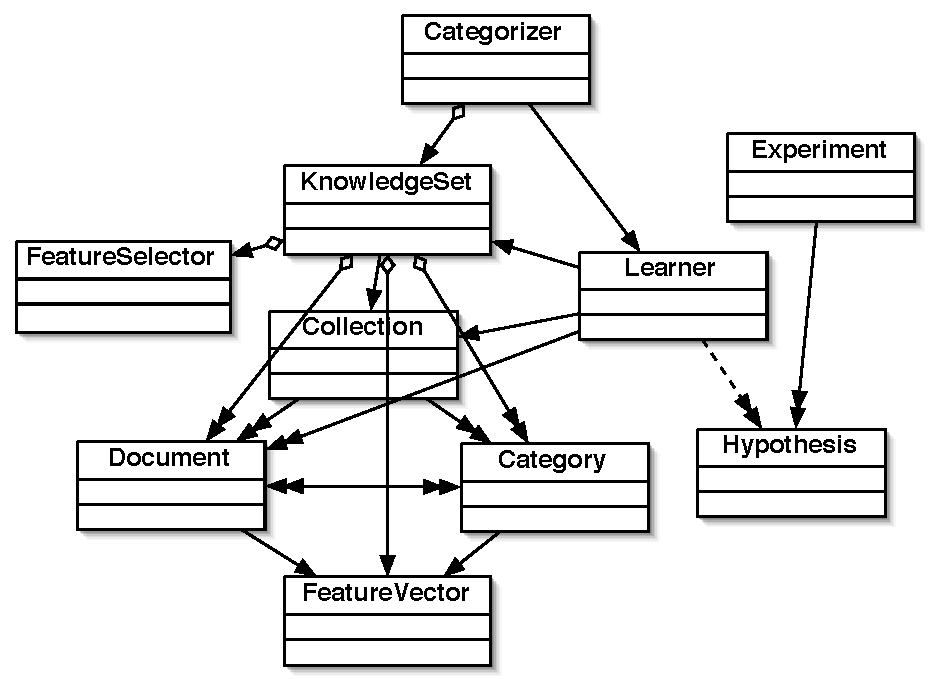
\includegraphics[width=\linewidth]{figures/classes-uml.pdf}
\caption{Class composition diagram for \aicat}
\label{classes-uml}
\end{figure}

Some examination of the basic relationships between classes and the
responsibilities of each class is helpful before looking at the design
in more detail.  The major classes in the \aicat\ framework
are:

\begin{description}

\item[KnowledgeSet]

The \class{KnowledgeSet} class represents a set of processed documents, a set
of categories, and a many-to-many mapping between the two sets.
Processing may involve tokenization, stopword removal, linguistic
stemming, feature selection, and vector weighting.  Note that the term
``knowledge set'' is somewhat unique to this project.

A \class{KnowledgeSet} contains references to many \class{Document} objects and
\class{Category} objects.  It uses \class{Collection} objects to instantiate \class{Document}
and \class{Category} objects.  It uses a \class{FeatureSelector} object to perform
feature selection.  It also contains a \class{FeatureVector} object
representing the features present in all documents.

\item[FeatureSelector]

Feature selection is performed by subclasses of the \class{FeatureSelector}
class.  Each \class{KnowledgeSet} object contains a \class{FeatureSelector}
object---the \class{KnowledgeSet} provides the information necessary to do
feature selection, and the \class{FeatureSelector} performs the desired
feature selection algorithm.

\item[Collection]

Because data sets in text categorization may be very large, and
because their documents may exist in several different underlying
storage mechanisms (e.g. as files in a filesystem, sections of a
larger XML file, or fields in a database), a \class{Collection} class provides
an abstract interface to a set of stored documents, together with a
way to iterate through the set and return \class{Document} objects.

A \class{Collection} object may be used in several contexts within the
framework.  For instance, a \class{KnowledgeSet} instantiates its Document and
\class{Category} objects through a \class{Collection} object.  A \class{Learner} object may
also mass-categorize the \class{Documents} in a \class{Collection} object.

\item[Document]

Each text document is represented by a \class{Document} object, or an object
of one of its subclasses.  Each document class contains methods for
turning document data into a \class{FeatureVector}.  Each document also has
a method to report which categories it belongs to.

\item[Category]

Each category is represented by a \class{Category} object.  Its main purpose
is to keep track of which documents belong to it, though it also
contains methods for examining statistical properties of an entire
category.

\item[Learner]

The abstract \class{Learner} class provides an interface to train on a
set of pre-categorized documents and subsequently categorize
previously unseen \class{Document} objects.  Its
concrete subclasses implement specific categorization algorithms like
\naive\ Bayes, SVM, Decision Tree, and so on.

\item[FeatureVector]

Most categorization algorithms don't deal directly with documents'
data, they instead deal with a \emph{vector representation} of a
document's features.  Most often, documents are represented using the
``Bag of Words'' model \cite[p. 10]{sebastiani:02}, i.e. a non-ordered, weighted set of
features.  The \class{FeatureVector} class provides an interface to the
operations one may perform on these vector representations, such as
querying features' presence or absence in a document, adding vectors
to each other, and so on.

\item[Hypothesis]

The result of asking a \class{Learner} to categorize a previously unseen
document is a \class{Hypothesis} object.  It may be queried for information
about which categories were assigned, which category was the single
most appropriate category, what scores were assigned to each category,
and so on.

In order to support this range of behaviors, the \class{Learner} is
required to create the \class{Hypothesis} object by specifying an
appropriateness score for each category and a threshold for category
membership.  Any category whose score is above the threshold is
considered assigned by the system to the given document.

\item[Experiment]

The \class{Experiment} class can examine the results of many categorization
decisions (i.e., many \class{Hypothesis} objects) and may be queried for
aggregate information about the results.  This is often used in order
to determine the quality (as measured by precision, recall, error,
etc.) of a \class{Learner} on a collection of test documents.

\item[AI::Categorizer]

An umbrella class \aicat\ sits above the rest of the classes,
providing a convenient interface to a complete system for text
categorization.  Most applications built using the framework will
instantiate an object of this class.  Note that the term \aicat\ can
refer either to the framework as a whole, or to the umbrella class.
The distinction will be made clear in this text where it is necessary
to do so.

\end{description}

\section{Design Patterns in \aicat}

The real power and intellectual content of any framework lies not in
the design of its individual classes, but in the interfaces between
the classes and the way objects collaborate to solve problems in the
framework's application domain. \cite[p. 31]{fayad:99} These
relationships can be quite complicated and difficult to explain, yet
understanding them is essential to understanding the framework.

In order to shed light on the design of complex object-oriented
systems, many researchers and software developers have tried to
standardize language and notation for class and object relationships.
There is as yet no universally accepted terminology for describing
these relationships, but one common practice is to use so-called
``design patterns'' to provide a baseline grammar for discussing
commonly seen patterns of cooperation in object-oriented
design. \cite[p. 3]{gamma:95} The design patterns do not provide
prescriptions for software design, but rather descriptions of best
practices in common situations.  Most design patterns in
\cite{gamma:95} include discussions of various trade-offs in their
application, indicating that a design pattern is actually a family of
similar solutions to a problem, not one rigid solution.

In this section, certain important local structures in the \aicat\
framework design will be discussed using the language of design
patterns.  The ``Iterator,'' ``Composite,'' ``Adapter,'' ``Strategy,''
and ``Factory Method'' patterns are discussed, and specific examples
from \aicat\ show how they are applied within the framework.  These
are not by any means the only instances of common design patterns in
the framework, nor do the specific patterns in \cite{gamma:95} provide
a complete catalog of all possible patterns in software.  This
discussion also does not give complete coverage to all design-related
issues involved in \aicat.  But patterns often provide a starting
point for design discussion, and their use has been found beneficial
in many diverse arenas \cite{granlund:99}, so they are used here in
the hope that they clarify the important design issues.

\subsection{Iterator}

The Iterator pattern provides ``a way to access the elements of an
aggregate object sequentially without exposing its underlying
representation.'' \cite[p. 257]{gamma:95} Its main purpose is to
decouple the traversal process on an object's aggregate members from
the object's internal data structure implementation.  In this way,
clients can iterate through aggregate objects without knowing the
objects' internal structure.

In the \aicat\ framework, it is often necessary to iterate
through collections of documents and perform some action on them.  For
example, the documents may form a training set for a \class{Learner} to base a
model on, or they may form a test set on which to evaluate the model.

The \class{Collection} class implements the Iterator pattern
\cite[p. 257]{gamma:95} over documents in the framework.  Figure
\ref{Iterator-collection} shows the main relationships involved in
this pattern.

\begin{figure}
\includegraphics[width=\linewidth]{figures/Iterator.pdf}
\caption{The Iterator pattern in the \class{Collection} class}
\label{Iterator-collection}
\end{figure}


\cite[p. 259]{gamma:95} suggests that the most common reasons for
using a formal custom iterator are:

\begin{itemize}

\item to access an aggregate object's contents without exposing its
internal representation.

\item to support multiple traversals of aggregate objects.

\item to provide a uniform interface for traversing different
aggregate structures.

\end{itemize}

The first and third reasons are most germane to the TC document iteration
process.  As explained in section \ref{Document storage}, it is
important that the framework can directly import documents from their
various underlying storage mechanisms in order to prevent unnecessary
duplication of data.  In order to hide the details of the storage
mechanism from the rest of the framework, a \class{Collection} object
retrieves documents from the storage mechanism and returns them
as \class{Document} objects.  It provides a unified interface to iteration
over stored documents so that the various classes that need to perform
this iteration (chiefly \class{Learner} and \class{KnowledgeSet}) don't need to be
aware of storage issues.  In this sense, the ``internal
representation'' of the aggregate structure is often external to the
framework itself---it may be files in a filesystem, entries in a
database, records in an XML document, or another mechanism.

In addition to providing a generic interface to a stored collection of
documents, the Iterator pattern allows clients of the \class{Collection} class
to use memory efficiently.  A \class{Collection} object will typically defer
creation of its \class{Document} objects until its client calls its
\method{next} method.  In this way, the \class{Collection} doesn't store all
the \class{Document} objects in memory simultaneously---if the client needs to do so,
it can, or it can merely query properties of each document and dispose
of them in turn.

Note that the \class{Collection} class defines a \method{next} method,
but no \method{previous} method.  This is largely because common
document storage mechanisms like filesystems or databases typically
only have one-directional iterators.  Insisting that
\class{Collection} classes needed to implement a \method{previous}
method to support bi-directional iteration would impose an
unreasonable burden on them.

In order to decouple the storage mechanism from the internal format of
documents (see section \ref{Document format}), \class{Collection}
classes can cooperate with any subclass of the \class{Document} class.
The client of the \class{Collection} class informs it that it should
instantiate documents using a certain \class{Document} subclass.
Since the \class{Document} subclasses share a common interface, \class{Collection}
may remain ignorant of all internal document formatting issues,
passing data to the proper constructors in order to instantiate
\class{Document} objects.


\subsection{Composite}

The Composite pattern ``lets clients treat individual objects and
compositions of objects uniformly.'' \cite[p. 163]{gamma:95} It is
often used to represent trees or other data structures in which the
form of a subset of the structure is not qualitatively different from
the form of the entire structure.  In simple terms, this means that
the same kinds of operations---iteration over sub-nodes, inspection of
the root node, and so on---can be performed on the entire tree, a
subtree, or even a single node.

In fact, the Composite pattern does not apply only to tree
structures.  It applies whenever a self-similarity exists between the
whole and the parts in a part-whole hierarchy.

One instance of this kind of structure in Text Categorization is in
so-called ``ensemble learners,'' also known as ``classifier
committees.''  An ensemble learner is a categorizer that combines the
results of a set of other categorizers in some way to arrive at a
categorization result of its own. \cite[p. 30]{sebastiani:02} Often,
an ensemble learner may outperform each of its constituent members on
the general categorization task.  \cite{tumer:98}

To implement ensemble learners within \aicat, the Composite
pattern may be applied to the \class{Learner} class to create a
\class{Learner::Ensemble} subclass.  Figure \ref{Composite-ensemble}
shows the classes participating in this pattern.

\begin{figure}
\includegraphics[width=\linewidth]{figures/Composite.pdf}
\caption{The Composite pattern in the \class{Learner::Ensemble} class}
\label{Composite-ensemble}
\end{figure}

Since \class{Learner::Ensemble} is a subclass of the abstract
\class{Learner} class, it conforms to the \class{Learner} interface.
This is crucial to implementation of the Composite pattern---it means
that clients may use the \class{Learner::Ensemble} class without
knowing that it implements an ensemble learner behind the scenes.  In
this way, transparent ensemble learning is achieved through
polymorphism.

According to \cite[p. 30]{sebastiani:02}, ensemble learning techniques
can be specified by (1) a set of individual learners (the ``members''
in Figure \ref{Composite-ensemble}), and (2) a mechanism for combining
the output of the individual learners.  The \class{Learner::Ensemble}
class can provide generic support for creating the member learners of
the ensemble, but the combination mechanism may take many different
forms.  Such algorithms are an active area of Machine Learning
research.  As such, \class{Learner::Ensemble} may be subclassed in
order to implement different combination mechanisms.  Since these
subclasses implement the combination algorithm in different ways, they
may themselves be seen as carrying out a Strategy pattern (see section
\ref{Strategy}).


\subsection{Adapter}

The Adapter pattern ``converts the interface of a class into another
interface clients expect.'' \cite[p. 139]{gamma:95} It is commonly
used when an existing resource provides the functionality necessary
for a certain task, but the interface of that resource doesn't match
the interface necessary for the environment in which that task must be
performed.  For example, a framework may require that a particular
role is implemented by subclasses of a certain abstract class.  This
helps unify functionality by taking advantage of polymorphic
abstraction. \cite[p. 5]{fayad:99} That functionality may already be
present in an existing body of code outside the framework.  An Adapter
can help bridge the gap between the two code bodies by letting the
external code function inside the framework.\footnote{An Adapter may
sometimes be called a Wrapper.  Both terms will be used in this
discussion.}

Many developers in the text categorization community create their
software as demonstrations of novel algorithms, or as stand-alone
libraries that implement one small part of the overall text
categorization task.  The majority of cutting-edge research will be
implemented in this way, if a public implementation is available at
all.  In order to leverage this work for a categorization framework,
some adaptation is invariably necessary.  Unless a developer happened
to be using \aicat\ as a development environment, her implementation
will not be directly usable as a framework element.  Thus Adapters
provide a mechanism for keeping the framework current with advances in
the field of text categorization.

\begin{figure}
\includegraphics[width=\linewidth]{figures/Adapter.pdf}
\caption{The Adapter pattern in the Learner class}
\label{Adapter-learner}
\end{figure}

Figure \ref{Adapter-learner} shows how the Adapter
pattern is present in \aicat's \class{Learner} class.  The abstract
\class{Learner} class specifies a common interface that all subclasses
must conform to.  Several of its concrete subclasses implement their
functionality using a framework-external resource.  For example,
\class{Learner::DecisionTree} uses the stand-alone module
\class{AI::DecisionTree} for implementation.  \class{Learner::Weka}
is a wrapper around the ``Weka'' Machine Learning system.
\class{Learner::SVM} is a wrapper around a framework-external
\class{Algorithm::SVM} module, which is itself a wrapper around the
\texttt{libsvm}\cite{libsvm} C library.\footnote{Note that
\class{Learner::SVM}, Weka, and \texttt{libsvm} are not part of the
contributed work of this thesis, as they are written by other authors.}

Note that these four Adapter examples exhibit three very different
applications of the Adapter pattern.  \class{Learner::DecisionTree}
exhibits a very straightforward Adapter usage as presented in
\cite{gamma:95}---an existing stand-alone class exists that implements the
needed functionality, and its interface is adapted to the framework
requirements by a simple wrapping subclass.  The \class{Learner::SVM}
wrapper is also fairly straightforward.  However, the other two
wrappers exhibit well the highly heterogeneous nature of the text
categorization domain.  The main reason for the adaptation in the
\class{Algorithm::SVM} class is to provide a Perl interface to a C
library.  The \class{Learner::Weka} adapter combines language
adaptation (in this case, Java to Perl) with functionality
transformation (mapping Weka's methods to the required \class{Learner}
interface).

Adapters can create design flexibility.
The current implementation of \class{Learner::Weka} interfaces with
Weka through its command-line interface, but this is not a design
constraint.  Future implementations may embed the Weka system inside
the \class{Learner::Weka} module for reasons of efficiency or platform
compatibility.  Because this interface is hidden using an Adapter
pattern, the implementation may be changed freely.

The differences in interfaces between the Adapter and the Adaptee may
be merely historical, or they may reflect different needs in different
domains.  The Adapter must conform to the interface of its abstract
superclass, which is typically designed to be independent of subclass
abilities and implementations.  The Adaptee may be designed for use in
a different arena, with extra functionality, or an interface that
takes full advantage of its capabilities.

Using Adapters may bring major benefits in the area of reusability.
Obviously, classes won't have to be re-implemented if the
functionality can be adapted from an existing implementation.  Second,
and perhaps more importantly, classes initially implemented for a
framework may be converted into Adaptee classes, usable in isolation.
This can bring them better exposure in other projects and thus more
feedback, maturing them quickly.  This can be a major win, because
iteration is considered a limiting factor in framework development
\cite[p. 75]{fayad:99}, and any process that speeds up maturity in
framework components can have a large impact.  Adapters can also force
a more robust encapsulation of design in the Adaptee, bringing
benefits in the conceptual and technical segmentation of the
framework.

\subsection{Strategy}
\label{Strategy}

The Strategy pattern defines ``a family of algorithms, encapsulates
each one, and makes them interchangeable.'' \cite[p. 315]{gamma:95}
It is used when a domain task needs to be carried out, but there may
be several ways to carry out that task, and it is important to let the
user or client choose from among these alternatives.

An important concept in the Strategy pattern is that of ``behavior.''
In \cite{gamma:95}, the Strategy pattern is recommended when ``many
related classes differ only in their behavior.''  In this context, a
distinction is made between an algorithm's purpose and its behavior.
For example, a set of algorithms for finding line-break points in text
paragraphs have a common purpose (to accomplish the line-breaking
task), but they may carry out their task in different ways.  The
algorithms may make different trade-offs in terms of speed and memory,
or they may try to optimize different aspects of the task.  Since it
is impossible to satisfy all clients in all situations with a single
choice of algorithm, it is desirable to encapsulate each algorithm in
a class that can be chosen or extended by the client.

The field of text categorization has several natural applications for
the Strategy pattern.  One of the primary concerns of most TC
researchers is the development of novel algorithms for various aspects
of the categorization task, so it is essential for these algorithms to
be easy to vary in a categorization framework.  In the language of
\cite{fayad:99}, these algorithms are framework ``hot spots.''

The most obvious Strategy application in \aicat\ is the
\class{Learner} class and its subclasses.  These classes all have a
common task to perform, that of training a categorizer and
categorizing unseen documents.  The various subclasses represent very
different ways to accomplish that task.  Importantly, the results of
the task, and not just the internal mechanism that performs it, may be
different depending on which \class{Learner} subclass is used.

\begin{figure}
\includegraphics[width=\linewidth]{figures/Strategy.pdf}
\caption{The Strategy pattern in the Learner class}
\label{Strategy-learner}
\end{figure}

Figure \ref{Strategy-learner} shows how the Strategy pattern appears
in the \class{Learner} class and its subclasses.  Three concrete
subclasses are shown that implement specific Machine Learning
algorithms (see Figure \ref{inheritance-uml} for other \class{Learner}
subclasses currently implemented).  From the point of view of the
client \aicat\ object, all \class{Learner}s have the same interface,
and may therefore be treated uniformly.  The framework user or
application designer, however, may choose judiciously among subclasses
depending on the particular needs of the application.  Customizability
of the Machine Learning algorithm is of paramount importance to the
framework, since it would be useless to most researchers if this were
not the case.  Many researchers may wish to write their own
\class{Learner} subclasses, using this portion of the framework in the
``whitebox'' paradigm.  Other researchers, and most application
developers, will want to use existing framework classes in a
``blackbox'' framework usage style. \cite[p. 10]{fayad:99} Either
method is supported.

Each \class{Learner} subclass must implement the abstract
\method{train} and \method{categorize} methods in order to perform the
two essential tasks of any \class{Learner}.  The \method{train} method
examines a \class{KnowledgeSet} object and builds an internal (and
opaque) model that will be used to categorize future documents.  The
\method{categorize} method takes a \class{Document} object as an
argument and returns a \class{Hypothesis} object representing the
outcome of categorization based on the model.

\begin{figure}
\includegraphics[width=\linewidth]{figures/Strategy-feasel.pdf}
\caption{The Strategy pattern in the FeatureSelector class}
\label{Strategy-feasel}
\end{figure}

Another application of the Strategy pattern is shown in Figure
\ref{Strategy-feasel}.  Here, the varying algorithm performs
feature selection, another framework hot spot.  There has been much
activity in current research on improving feature selection for
different scenarios \cite{yang:01,yang:97}, so customization in this
area is also essential.

To perform feature selection, a \class{KnowledgeSet} object invokes
either the \method{select\_features} or \method{scan\_features} method
of the \class{FeatureSelector} object, depending on whether a complete
\class{KnowledgeSet} or a \class{Collection} object should be
examined.  Examining a \class{Collection} iteratively requires less
memory because the documents don't have to be loaded into memory all
at once, but it requires a separate pass through the data.  The choice
of which method to run is made in response to user specification.

Because \method{select\_features} and \method{scan\_features} are
virtual methods in the parent class, any concrete subclass must
implement these methods according to the particular algorithm the
subclass represents.  As of this writing, only the
\class{FeatureSelector::DocFrequency} subclass is implemented, but
the other subclasses in the diagram are planned.


\subsection{Factory Method}
\label{factory-method}

In any framework of sufficient size and customizability, attention
must be paid to the issue of how specific classes are chosen for the
various framework roles, how these classes are instantiated, and how
the instantiated objects are connected to each other.  In the simplest
possible case for the framework developer, the framework client code must create all objects and
manually connect them to each other---for instance, in \aicat, the
client code might create a \class{KnowledgeSet} object, a
\class{Learner} object, an \aicat\ object, a \class{Collection}
object, then populate the \aicat\ object with \class{KnowledgeSet} and
\class{Learner} objects, and the \class{KnowledgeSet} with a
\class{Collection}, thus satisfying the structural relationships
indicated in Figure \ref{classes-uml} on page \pageref{classes-uml}.
An approach like this is diagrammed in Figure
\ref{naive-constructors}.

\begin{figure}
\includegraphics[width=\linewidth]{figures/naive-constructors.pdf}
\caption{A client-side approach to object construction}
\label{naive-constructors}
\end{figure}

This approach works, but it is error-prone and cumbersome.  It forces
every client to specify the framework relationships explicitly, when
in fact these are fundamental relationships of the \emph{framework},
not of the client code.  It makes little sense for this structural
code to be outside the framework, and even less sense for it to be
duplicated in every application that uses the framework.  Note too
that Figure \ref{naive-constructors} only shows a small part of the
framework being used---in reality, the client code would have to
accept responsibility for creating all the objects in the framework,
not just the four pictured here.

For these reasons, it is often better if the framework can provide
support for object creation and enforcement of the framework
relationships.  An example of this situation is pictured in Figure
\ref{better-constructors}.  Here, the patterns of object creation more
closely follow the class relationships that will be used at runtime.
This design is moving closer toward a factory-style pattern, in which
object creation is delegated to another object. \cite{gamma:95}
defines two specific kinds of factory patterns, ``Factory Methods''
and ``Abstract Factories.''  Figure \ref{better-constructors} does not
fit either of these patterns exactly, but it does fall under the
general category of factory object creation.

\begin{figure}
\includegraphics[width=\linewidth]{figures/better-constructors.pdf}
\caption{A framework-side approach to object construction}
\label{better-constructors}
\end{figure}

A scheme like that in Figure \ref{better-constructors} has both
advantages and disadvantages compared with that in Figure
\ref{naive-constructors}.  One obvious advantage is that the client
code is greatly simplified, because it needn't create any framework
objects except the top-level object, and because it doesn't have to
link the objects to each other.  This eliminates redundancy in
multiple client code bases, and allows the framework designer greater
flexibility in redesigning the framework hierarchy.  Another advantage
is that the framework objects are created by the objects that use
them, so class code can accept responsibility for its subordinate
objects' entire life cycles.

However, these properties can also be seen as disadvantages.  If each
framework object assumes all responsibility for creating its
subordinate objects, then the client may not be able to control the
creation process effectively.  This is a problem for at least two
important reasons: first, the client may wish to change some
properties of the objects it creates.  If it passes all constructor
parameters to the top-level class constructor, then this constructor
must have knowledge of all of its subordinate classes' parameters in
order to affect their construction correctly.  This would couple the
framework classes too closely.  Second, the client may (and frequently
will) change which classes are participating in the framework
hierarchy.  If the \class{KnowledgeSet} class always creates a certain
class of \class{Collection} object, then in order to substitute a
different \class{Collection} class, the \class{KnowledgeSet} class
would need to be subclassed---and the top-level \aicat\ class would
need to be subclassed too, in order to create the new type of
\class{KnowledgeSet}, leading to a proliferation of subclasses just to
manage object creation.  Clearly a better solution is needed.

In order to create a proper solution, some analysis of the problem is
warranted.  Part of the reason these creational issues are difficult
is that no standard method exists to translate the framework's design
relationships into code.  Common programming languages have no
built-in support for managing the patterns of creation necessary in
frameworks.  Contrast this with inheritance relationships, which are
directly supported by object-oriented languages.  For instance, a C++
or Java \texttt{class} declaration lists its superclasses explicitly,
and Perl specifies inheritance via each class's \texttt{@ISA} array.
Because inheritance is directly implemented by the language, it is
easy for framework users to understand inheritance relationships, and
these relationships are expressed straightforwardly in the framework
code.  For support of this point, consider object-oriented programming
in languages like C that don't have inherent OO support, where
understanding the inheritance structures can be much more
challenging.\cite[p. 7]{fayad:99}

With this perspective in mind, one solution is to create a way for
each class to explicitly declare its constructor parameters and its
relationships to other classes, and then let the framework manage
object creation in a consistent, centralized manner based on these
declarations.  In a sense, this approach extends the implementation
language to be able to express the important framework relationships
directly, rather than letting them emerge implicitly from patterns of
usage in the code.  Client code then supplies parameters that inform
the top-level object about which classes should be instantiated and
what parameters should be passed to each class's constructors, and the
framework itself directs object the creation process.

\begin{figure}
\includegraphics[width=\linewidth]{figures/factory-constructors.pdf}
\caption{A centralized approach to object construction}
\label{factory-constructors}
\end{figure}

Because many users of an application framework will be hesitant to
depend on a modified, nonstandard version of the implementation
language, \aicat\ uses inheritance to add these explicit declaration
capabilities to every class participating in the framework hierarchy.
Figure \ref{factory-constructors} shows an example of how this
inheritance functions.  The abstract \aclass{ObjectFactory}
class\footnote{The \aclass{ObjectFactory} name is used here only for
discussion purposes.  See Section \ref{constructor-methods} for the actual
implementation details.} adds the ability for any class derived from
it to declare the relationships discussed in the previous paragraph.
It also manages the creation of subordinate objects.  For instance,
the top-level \aicat\ class declares that it contains both a
\class{KnowledgeSet} and \class{Learner} object in an aggregation
relationship.  When an \aicat\ object is created, \class{KnowledgeSet}
and \class{Learner} objects will automatically be created by the
\aclass{ObjectFactory} according to the client code's parameters.  The
\class{KnowledgeSet} also declares that it will need to create
\class{Collection} objects on demand, and calls creational methods
provided by its \aclass{ObjectFactory} superclass when it needs to
create them.

It is important to note that this is not a direct application of
either the Factory Method or Abstract Factory patterns in
\cite{gamma:95}.  The standard Factory Method pattern requires
separate subclasses to create the concrete subclasses.  A closer
variation is the ``Parameterized Factory Method''
\cite[p. 110]{gamma:95}, which lets the specific subordinate class
be determined by switching among several known classes.  This is
closer to the data-driven approach employed in \aicat, but doesn't
address the issue of how the subordinate classes must actually be
created at runtime.  The Abstract Factory pattern is also similar in
that the creation of multiple objects is centralized, but in \aicat\ a
separate factory object is not necessary.

This approach effectively solves the problems with the first two
approaches considered here.  The client code is freed from having to
create multiple framework objects, and the framework relationships are
expressed explicitly in the framework code, not in the client code or
implicitly in the framework implementation.  Clients are also able to
easily change which classes participate in the framework hierarchy,
and can specify constructor parameters without invoking the
constructors directly.  Framework code doesn't create subordinate
objects directly, but defers creation to factory methods inherited
from superclasses.  In this way, subclassing is kept to a minimum, and
the framework runtime structure can be highly parameterized.

\section{Limitations}

In any software design process, choices must be made that determine
the scope and direction of the project.  In designing \aicat, these
choices have been made in a way that tries to maximize usefulness for
the intended audience, reuse of framework components, framework
efficiency and flexibility, and rapid application development.  In
some cases, these decisions may limit the capabilities of the
framework.  This section describes some of these limitations, explains
the reasons for them, and proposes alternative ways to deal with the
problems they present.

\subsection{Structured Feature Vectors}

The basic data model representing documents in the \aicat\ framework
is the feature vector.  In this model, certain features of each
document (typically counts of words or word stems) are measured, and
their values are represented as vectors in a vector space encompassing
all document vectors in the training set.  Each document vector is
\emph{flat}, i.e. an $n$-dimensional vector with no internal
structure, where $n$ is the total number of features in all the
training documents.  This representation has been shown to be very
effective for Text Categorization applications
\cite[p. 10]{sebastiani:02}, and is crucial for such common TC
algorithms as k-Nearest-Neighbor and Support Vector Machines.

However, many environments routinely use richer data models for
documents.  For instance, researchers in the Linguistics community
often represent documents as hierarchical data structures indicating
each syntactical element's relationship to the other syntactical
elements in the document.\cite[ch. 11 \& 12]{manning:99} \cite{sag:99}
Additionally, many structured HTML and XML business documents are
represented using the Document Object Model, which provides a common
programmatic interface to the logical structure of
documents.\cite{dom}

Because few TC techniques in the common literature take advantage of
document structure, and because several techniques depend on
unstructured vector representations, the \class{FeatureVector} class
only provides an interface to unstructured feature vectors.  This
class does leave the \emph{implementation} of the vectors unspecified,
however, so that different internal representations are possible (see
Section \ref{imp-featurevectors} for more on this topic).

In an application using structured documents, two options exist for
taking advantage of this structure using \aicat.  One option is to
``flatten'' the structure of the document into a traditional feature
vector representation. (XXX - need to explain further, with
references)  

Another option if the document structure is just a sequence of
document sections and not arbitrarily nested structures is to use the
\aicat\ framework's \param{content\_weights} parameter.  This allows
each document to be divided into an arbitrary number of sections such
as title, abstract, body, and so on, assigning ``importance'' weights
to each section.  These weights will be used when creating a feature
vector from the document content, in effect automatically flattening
the document into a traditional feature vector.

Neither of these two solutions allow the framework to truly deal with
arbitrarily structured documents in any natural way.  It is therefore
to be understood that the framework is not currently capable of
exploiting this structure very deeply, and this is a possible area of
future work.

\subsection{Hierarchical Categorization}

Hierarchical categorization is the process of categorizing documents
into a set of categories possessing a treelike structure.  The
hierarchical nature of the category set may be exploited for both
increased efficiency and improved accuracy.\cite{dumais:00}  Because
some common categorization problems are inherently hierarchical, the
field of hierarchical categorization has seen significant attention in
the research literature.\cite[p. 7]{sebastiani:02}

In the \aicat\ framework, hierarchical categorization has not
explicitly been supported in the architecture.  The set of categories
in any framework categorization task is assumed to be a simple list of
named sets of documents, with no hierarchical structure.  However,
there are at least two ways of dealing with hierarchical
categorization tasks using the framework.

The first way is to simply transform the hierarchical set of
categories into a simple flat list, by prepending each category's name
with the names of all its parent categories.  In this way, the
framework will assign any category in the flat list of categories, and
then the results can be transformed back into members of the
hierarchical category set.  The main advantage of this technique is
that it is simple to apply, with a natural and transparent
transformation between structured and flat category sets.  The main
disadvantage is that the system is not really performing hierarchical
categorization at all, so it is not taking advantage of any of the
hierarchical category structure for efficiency or accuracy
improvements.

The second way to achieve hierarchical categorization using \aicat\ is
to manually break the categorization task into several smaller tasks,
building a separate machine learner for each splitting node in the
category hierarchy.  This is a common approach to hierarchical
categorization in the literature
\cite{dumais:00,koller:97,chakrabarti:98}, and seems a natural mapping
of the hierarchical problem into a hierarchical solution.  The main
disadvantage with this method is that the framework provides no direct
support for creating a hierarchy of categorizers and using them for
categorization, so the client must create and maintain code for the
hierarchical aspect of the task.  This is another possible area of
future work, and another student in the Web Engineering Group at
Sydney University is currently working toward a solution for using
\aicat\ in hierarchical categorization.
